\chapter{Implementation} % (fold)
\label{chap:Implementation}
This chapter focuses on the implementation of our experiment.
Initially, \autoref{sec:Protocol Specification} presents the implemented
    \gls{mead} specification.
Subsequently, \autoref{sec:Router} delves into the technical details of the
    Kernel implementation of the router software.
\autoref{sec:Sender} provides insights into the sender implementation, including
    the interaction of discovery and data delivery phases and the receiver
    grouping algorithm.
Finally, \autoref{sec:Experiment} demonstrates our designed network topologies,
    deployment of the testbed, and the conduction of the experiment.

\section{Protocol Specification} % (fold)
\label{sec:Protocol Specification}
Since the existing literature on \gls{mead} \cite{meadcast1,meadcast2} lacks
    specific details regarding the header, such as specific field sizes or
    content (see \autoref{sub:MEADcast}), in this section we introduce the
    specifications utilized for our experiments.

Firstly, we omit the usage of an empty Hop-by-Hop IPv6 extension header as
    introduced by \citeauthor{meadcast1} \cite{meadcast1, meadcast2}.
We do this for several reasons:
First, to reduce the overhead of \gls{mead}.
Second, if a non-\gls{mead} router attempts to process Hop-by-Hop extension
    headers the packet probably ends up in the router's slow path
    \cite{rfc7045}, potentially harming the protocol's performance.
Third, since the \gls{mead} header is intended to be processed exclusively by
    \gls{mead} routers, over which we maintain control, the Hop-by-Hop
    extension header serves no purpose.
Lastly, according to various research studies, packets containing a Hop-by-Hop
    extension header experience an increased drop rate of up to 40\% compared
    to packets without an extension header \cite{rfc7872_ext_hdrs_drop_rate},
    especially across multiple \glspl{as}
    \cite{rfc9098_ext_hdrs_op_impl, rfc9288}.

Next, we introduce the detailed characteristics of the \gls{mead} header in our
    implementation.
The first four octets of the \gls{mead} header constitute the static routing
    extension header, which is shared by all routing variants.
This differs from previous implementations of \gls{mead}, which omitted the
    \textit{Segments Left} field \cite{sdn_ba}.
We decided to include this field to comply with RFC 8200
    \cite{rfc8200_ipv6_hdr}, reducing the likelihood that intermediate nodes
    drop \gls{mead} packets due to a malformed routing header.
Since there is no existing \textit{Routing Type} designated for \gls{mead}, we utilize the
    experimental values of 253 and 254 in accordance with RFC3692
    \cite{rfc3692_ipv6_rt_type}.
The \textit{Segments Left} field remains fixed to zero and is never altered because,
    according to RFC 8200 \cite{rfc8200_ipv6_hdr}, intermediate nodes that do
    not recognize the employed \textit{Routing Type} value must ignore the routing
    header and proceed to process the next header.
An illustration of the \gls{mead} header layout can be found in
    \autoref{lst:meadcast_header}, along with an in-depth description of each
    field in \autoref{tab:meadcast_header}.
Due to the time frame of this thesis, we omit the usage of the optional port
    list as it does not affect the core \gls{mead} processing.

\begin{figure}[!htbp]
\centering
\begin{bytefield}[bitformatting=\tiny,bitwidth=1.1em,boxformatting=\centering\small]{32}
\bitheader{0-31} \\
    \begin{rightwordgroup}{\small RT Hdr \\ \small Preamble}
    \bitbox{8}{Next Header} &
    \bitbox{8}{Hdr Ext Len} &
    \bitbox{8}{Routing Type \\ \tiny (Experimental: 253/254)} &
    \bitbox{8}{Segments Left \\ \tiny (0)}
    \end{rightwordgroup} \\
    \bitbox{8}{Num. Dst} &
    % \bitbox{2}{Fl.} &
    \bitbox{1}{\tiny D\\[-1.25pt] C \\[-1.25pt] V} &
    \bitbox{1}{\tiny R\\[-1.25pt]S\\[-1.25pt]P} &
    \bitbox{6}{Hops} &
    \bitbox{16}{Reserved} \\
    \bitbox{32}{Delivery Bitmap} \\
    \bitbox{32}{Router Bitmap} \\
    \wordbox[lrt]{2}{Address List \\ \scriptsize (variable length)} \\
    \skippedwords \\
    \wordbox[lrb]{1}{} \\
\end{bytefield}
\caption[Employed MEADcast header specification]{Employed \gls{mead} header specification}
\label{lst:meadcast_header}
\end{figure}

\bgroup
\begin{table}[!htbp]
\centering
\def\arraystretch{1.35}%  1 is the default
\setlength{\tabcolsep}{1.2em}
\begin{tabularx}{\textwidth}{lX}
\toprule
\textbf{Field}& \textbf{Description} \\
\midrule
Next Header   & A 8-bit selector, identifying the type of the immediately
                following header \cite{rfc8200_ipv6_hdr}.
                Employs identical values as the IPv4 Protocol field (e.g. 17 =
                UDP, 59 = No Next Header for IPv6)
                \cite{iana_prot_nums}.\\
Hdr Ext Len   & An 8-bit unsigned integer representing the length of the
                Routing header in 8-octet units, excluding the initial 8
                octets \cite{rfc8200_ipv6_hdr}. \\
Routing Type  & An 8-bit identifier denoting a specific Routing header variant
                \cite{rfc8200_ipv6_hdr}.
                Given the absence of an existing Routing Type for \gls{mead}, we
                utilize the experimental values of 253 and 254 in accordance
                with RFC3692 \cite{rfc3692_ipv6_rt_type}.\\
Segments Left & An 8-bit unsigned integer representing the number of remaining
                route segments, indicating the number of explicitly listed
                intermediate nodes yet to be traversed before reaching the
                final destination \cite{rfc8200_ipv6_hdr}.
                Remains fixed to zero and is not modified by \gls{mead} routers.
                Consequently, intermediate nodes that do not recognize the
                employed Routing type value are required to disregard the
                \gls{mead} header and proceed to process the subsequent header
                \cite{rfc8200_ipv6_hdr}.\\
Num. Dst.     & An 8-bit unsigned integer denoting the number of IPv6
                addresses encoded in the address list.
                The field size sets a theoretical limit of 255 destinations.\\
% Flags         & A 2-bit Bitmap. The highest-order bit classifies the packet
%                 either as a data (0) or discovery  (1) packet.
%                 The lowest-order bit indicates whether the packet is a
%                 discovery request (0) or response (1) \cite{meadcast2}.
%                 Valid combinations comprise \inlinelst{00}, \inlinelst{10}, and
%                 \inlinelst{11}\\
\makecell[l]{Flags\\\hspace*{2mm} Dcv \\\hspace*{2mm} Rsp \\\ } &
\makecell[X]{A 2-bit Bitmap, valid combinations comprise \inlinelst{00},
                \inlinelst{10}, and \inlinelst{11}.\\
                1 bit classifying the packet as a data (0)
                or discovery (1) packet.\\
                1 bit identifying the packet as a discovery request (0) or
                response (1) \cite{meadcast2}.}\\
Hops          & An 6-bit unsigned integer, specifying the distance between the
                sender and a router, denoted in the number of \gls{mead} hops.
                This field is utilized during the discovery phase. The sender
                initializes the field with zero, and it is incremented by each
                intermediate \gls{mead} router encountered.
                The field size sets a theoretical limit of 63 hops.\\
Reserved      & A 16-bit reserved field.
                Should be initialized to zero during transmission and
                disregarded upon reception.\\
Delivery Map  & A 32-bit Bitmap, where each bit at position $i$ indicates
                whether a router at index $i$ in the address list has already
                been delivered (0 = delivered, 1 = not yet delivered)
                \cite{meadcast2}. \\
Router Map    & A 32-bit Bitmap, where each bit at position $i$ indicates
                whether an address at index $i$ in the address list is a
                router (0 = receiver, 1 = router) \cite{meadcast2}.\\
Address List  & A variable-length list comprising the IPv6 addresses of
                receivers and \gls{mead} routers.
                The field size of the Delivery and Router Bitmap imposes a
                practical limit of 32 addresses.\\
\bottomrule
\end{tabularx}
\caption[Employed MEADcast header field description]{Employed \gls{mead} header field description}
\label{tab:meadcast_header}
\end{table}
\egroup

% section Protocol Specification (end)

\section{Router} % (fold)
\label{sec:Router}
This section provides an overview of the \gls{mead} router implementation in the
    Linux Kernel.
The \gls{mead} routing software is developed and tested using the latest stable
    Kernel release, version 6.5.3, at the time of development.
\gls{mead} routing capabilities are tightly coupled to the flow of IPv6 packets
    through the Kernel network stack, making it infeasible to create a separate
    Kernel module loadable at runtime.
Therefore, we decided to extend the IPv6 module with \gls{mead} capability.
This feature can be enabled or disabled at compile-time using the
    \inlinelst{CONFIG\_IPV6\_MEADCAST} flag.
To avoid the burden of recompiling or switching the kernel to enable or disable
    \gls{mead} support, we introduce a runtime configuration flag.
This flag is managed through Sysctl, providing the virtual file
    \inlinelst{/proc/sys/net/ipv6/meadcast/enable}, which contains either 0 for
    disabled and 1 for enabled (see \autoref{lst:rt_cfg}).
For instance, the root user can enable \gls{mead} support by running the command
    \inlinelst{"echo 1 > /proc/sys/net/ipv6/meadcast/enable"}.
However, it is crucial to ensure that this additional check does not adversely
    impact performance compared to a plain kernel, as it could potentially
    affect the reliability of experimental results.

Packets not designated to the router itself follow the ``forwarding'' packet
    flow in the Kernel.
IPv6 extension headers of these packets are normally ignored by the Kernel
    (except for the Router Alert extension).
Consequently, we embedded the entry point for \gls{mead} processing at the end of
    the \inlinelst{ip6\_forward} method located in
    \inlinelst{net/ipv6/ipv6\_output.c}.
If a packet contains the routing header extension the \inlinelst{mdc\_rcv}
    method located in \inlinelst{net/ipv6/mdcast.c} gets invoked.
This method performs basic sanity checks on the \gls{mead} header and then
    invokes \inlinelst{mdc\_dcv\_rcv} for discovery and
    \inlinelst{mdc\_data\_rcv} for data packets.

% discovery
% - validation
% - increment hop counter
% - clone socket buffer of incomming packet (discovery response)
% - update dst and src ip of discovery response
\textit{Discovery}: First, discovery packets get validated and the hop counter
    in the \gls{mead} header is incremented.
To create a discovery response the socket buffer struct of the incoming
    discovery request is cloned.
By this, we solely have to update the IP source and destination field of the
    cloned packet, set the response flag, and perform a routing table lookup
    for the sender's address.
The source IP address of the discovery response is set to the IP address
    associated with the interface returned from the routing lookup.
Lastly, the \inlinelst{dst\_output} method is invoked, dispatching the packet to
    the corresponding layer 2 handler.
The processing of the original packet does not need further handling, as it is
    already correctly done by the default forwarding flow.

\textit{Data}: Data packets undergo several steps upon arrival at the \gls{mead}
    router.
Firstly, they are validated, and the hop counter in the \gls{mead} header is
    incremented.
Subsequently, the router iterates over the Delivery and Router Bitmap to
    identify undelivered routers (indices set in both bitmaps).
During this iteration, if the router is not the last undelivered router in the
    sequence, the socket buffer of the original packet is cloned and forwarded
    accordingly.
However, if the router is the last undelivered router, the original packet can
    be forwarded without the need for costly replication.
To determine whether to clone the packet, the routers monitors whether an 
    undelivered router at index $r1$ has a successor (another undelivered
    router) at index $r2$, with $r1 < r2$.
The algorithm's specifics are depicted in \autoref{fig:router_hdr_parsing}.

For each undelivered router $R_u$ specified in the \gls{mead} header, the
    processing router $R_p$ decides whether to transmit the data via \gls{mead}
    or IP Unicast.
If the IP address of $R_u$ in the \gls{mead} header belongs to the processing
    router $R_p$ itself, all designated endpoints will be delivered via IP
    unicast.
Additionally, if the number of endpoints assigned to the considered router
    $R_u$ from the \gls{mead} header is below a certain threshold, the processing
    router $R_p$ performs a premature \gls{mead} to IP Unicast transformation.
For example, if $R_u$ has one designated endpoint, $R_p$ could execute a
    premature \gls{mead} to IP Unicast transformation, potentially enhancing
    performance.
The threshold can also be configured during runtime by setting the parameter
    \inlinelst{/proc/sys/net/ipv6/meadcast/min\_dsts}.
Setting \inlinelst{min\_dsts} to zero disables premature \gls{mead} to IP Unicast
    transformation.

If the packet is forwarded via \gls{mead}, the router updates both the delivery
    bitmap and the destination field of the IPv6 header.
In the delivery bitmap, all bits are set to zero except for the index
    corresponding to the considered router.
Additionally, the IP destination field is set to the address of the first
    receiver following the router in the address list.
Lastly, the router performs a routing table lookup for the new destination
    address and forwards the packet accordingly.

In case of IP Unicast transmission, the router converts the \gls{mead} packet
    into an IPv6 packet by copying the IPv6 header in front of the Layer 4
    header and adjusting the socket buffer pointers accordingly.
Additionally, in alignment with RFC 1624 \cite{rfc1624}, the L4 checksum is
    incrementally updated due to the modified destination IP address.

% Search for first router
%
% - validation
% - increment hop count
% - iterate bitmaps
%   - check which routers aren't delivered yet
%   - if router is not last undelivered router create a copy of socket buffer struct
%   - else use incoming one
% - forwarding
%   - if router addr in bitmap is of router or less than min_dsts eps -> m2u
%   - else: update bitmap (set all others to delivered), update ip dst field
% - m2u
%   - copy IP hdr in front of l3 header
%   - update skb pointers
%   - recalc checksum
\begin{figure}
    \begin{center}
        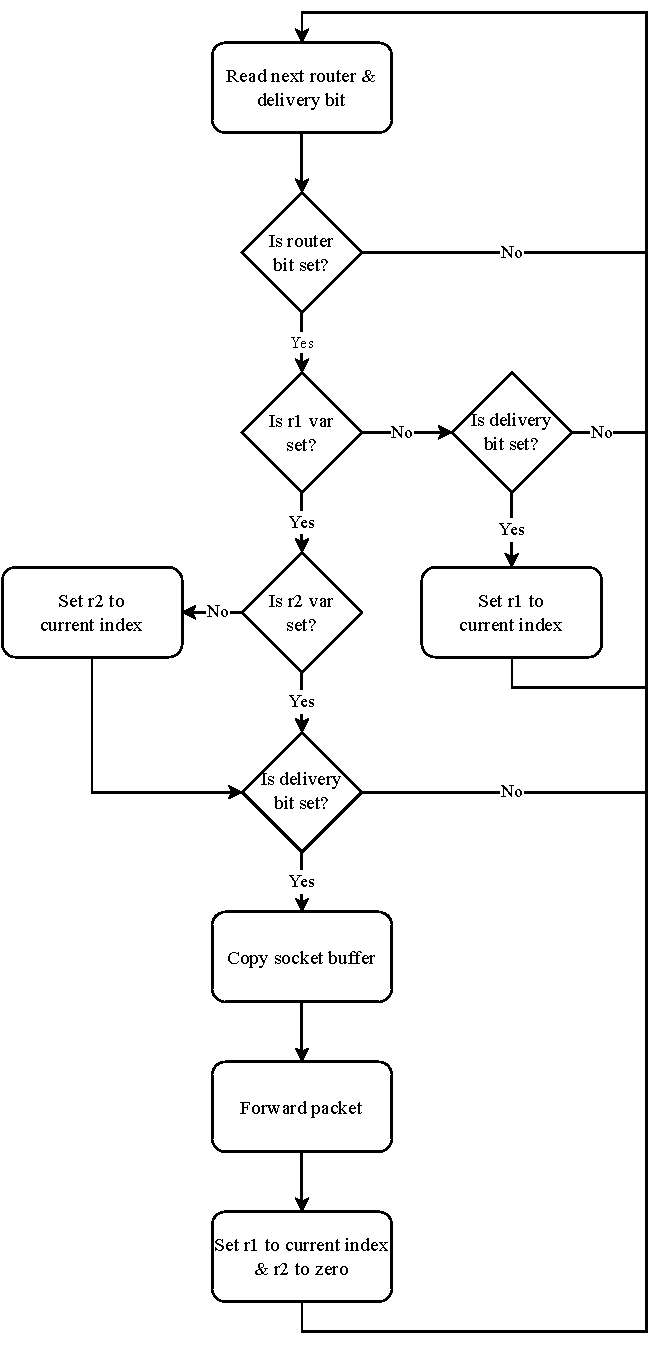
\includegraphics[scale=.85]{router_hdr_parsing.pdf}
    \end{center}
    \caption[Router: MEADcast header parsing]{Router: \gls{mead} header parsing}
    \label{fig:router_hdr_parsing}
\end{figure}

% \begin{figure}
%     \begin{center}
%         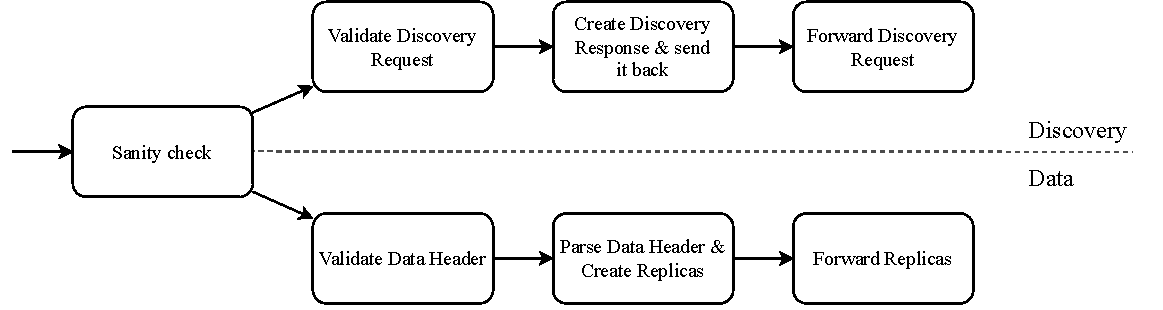
\includegraphics[width=\textwidth]{router_procedure.pdf}
%     \end{center}
%     \caption{\gls{mead} router procedure}
%     \label{fig:router_procedure}
% \end{figure}
% section Router (end)


\section{Sender} % (fold)
\label{sec:Sender}
This section provides an overview of our \gls{mead} sender implementation.
\autoref{sub:Sender Architecture} delves into the internal implementation
    specifics, such as threading and data structures.
\autoref{sub:Grouping} provides an introduction into the algorithm which
    groups a list of receivers into \gls{mead} packets.

\subsection{Software Architecture}
\label{sub:Sender Architecture}
To ensure efficient processing that is comparable to existing network
    protocol implementations, we chose to implement the sender in the C
    language.
The main tasks of the sender include sending periodical discovery requests to
    all group members, receiving discovery responses, constructing a topology
    tree based on the received discovery responses, grouping receivers into
    \gls{mead} packets, and transmitting data to all group members either via
    \gls{mead} or IP Unicast.

\paragraph{Startup} % (fold)
\label{par:Startup}
All receivers must be known at startup, dynamic runtime memberships are not
    supported.
We regard this decision as justifiable, given that \gls{mead} does not define any
    mechanism for joining or leaving a group, and the primary objective of this
    thesis is to compare the protocol with existing alternatives.
On startup the sender initializes a topology tree with itself as the root and
    all receivers as direct attached leaves.
Moreover, a TUN interface is created representing the common interface to other
    applications.
Any data, which is send to the TUN interface will be transmitted to the
    \gls{mead} group (see \autoref{fig:tun_dev}.
However, since \gls{mead} is a \textit{1:n} multicast protocol, the sender does not
    handle traffic directed from the \gls{mead} receivers towards the sender.
The \gls{mtu} of the TUN interface will be set to the MTU of the bind interface
    minus the maximum allowed \gls{mead} header size.
This ensures, that all packets read from the TUN interface can be transmitted
    via \gls{mead}.
Additionally, for convenience a host route to the TUN interface gets created 
    automatically (default: \inlinelst{fd15::1}).
Next, a discovery and transmission thread is created.
This is necessary to facilitate simultaneous data transmission and periodic
    \gls{mead} discovery.

\begin{figure}
    \begin{center}
        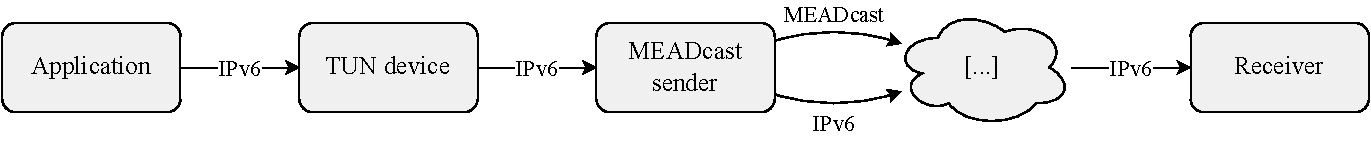
\includegraphics[width=\textwidth]{tun_dev.pdf}
    \end{center}
    \caption{Sender: TUN interface}
    \label{fig:tun_dev}
\end{figure}
% paragraph Startup (end)

\paragraph{TX thread} % (fold)
\label{par:TX thread}
The transmission thread operates on a straightforward pattern.
It reads data from the TUN device and transmits it to the \gls{mead} group either
    via \gls{mead} or IPv6 unicast.
The key element for data transmission is the \inlinelst{tx\_group} structure,
    which includes three members: \inlinelst{*mdc}, \inlinelst{nuni}, and
    \inlinelst{uni} (as detailed in \autoref{lst:txg_struct}).
These members encompass all the necessary information for data transmission,
    rendering \inlinelst{tx\_group} as the only data structure required by the
    transmission thread.
\inlinelst{*mdc} is a reference to a linked list of receivers grouped into
    \gls{mead} headers ready for transmission.
\inlinelst{nuni} contains the count of unicast addresses stored in
    \inlinelst{uni[]}.
Lastly, \inlinelst{uni[]} is an array of receivers served via IPv6 unicast.

The \inlinelst{tx\_group} structure is the only data accessed by both the
    discovery and transmisson thread.
Upon initialization of the transmission thread, a \inlinelst{tx\_group}
    structure is instantiated with all receivers added to the \inlinelst{uni[]}
    list and an empty \inlinelst{*mdc} list.
Subsequently, the \inlinelst{tx_group} is exclusively modified by the discovery
    thread.
To prevent race conditions on the \inlinelst{tx\_group}, the threads share an
    atomic reference pointing to the current group.

Next, the transmission thread enters an infinite loop executing the following
    steps.
Initially, it blockingly reads data from the TUN device.
Second, the sender atomically reads the current \inlinelst{tx\_group}.
This step is substantial because the \inlinelst{tx\_group} can be updated by
    the discovery thread at any time.
Finally, the data read from the TUN device is transmitted to the \gls{mead} group
    by first transmitting it via IPv6 unicast to all addresses listed in
    \inlinelst{uni[]} and subsequently transmitting it via \gls{mead} by copying
    the \gls{mead} headers stored in \inlinelst{*mdc} in front of the Layer 4
    header.
The copying of the \gls{mead} header overwrites the IPv6 header, necessitating
    the unicast transmission to occur before the \gls{mead} transmission.

\begin{listing}
\begin{minted}[linenos, frame=lines, framesep=2mm, breaklines]{c}
struct tx_group {
    struct child *mdc;
    size_t nuni;
    struct addr uni[];
};
\end{minted}
    \caption{Sender: tx\_group structure}
    \label{lst:txg_struct}
\end{listing}
% paragraph Tx thread (end)


\paragraph{Discovery Thread} % (fold)
\label{par:Discovery Thread}
% Discovery
% - Keep track of timers
% - Send and receive discovery
% - Perform grouping

% - init timer fd for discovery interval and discovery timeout
% - based on epoll (level-triggered)
% - enter infinitiv loop
%   - wait for an fd to become ready
%   - if interval:
%       - send discovery request to all group members
%       - disarms interval timer and enables timeout timer
%   - if mdc fd:
%       - receive discovery rsp, sanity checks
%       - modify topology tree (insert or update)
%   - if timeout:
%       - group receivers
%       - atomically update tx_group reference
%       - disarm timeout timer and enable interval timer
The discovery thread operates on a more intricate pattern compared to the
    transmission thread.
Its primary tasks include sending periodic discovery requests to all group
    members, receiving discovery responses from intermediate \gls{mead} routers,
    maintaining the topology tree, and grouping receivers into \gls{mead}
    headers.

To manage the recurring discovery phase, the sender utilizes a discovery
    interval and a discovery timeout timer (see
    \autoref{fig:discovery_timers}).
At the beginning of the discovery phase, the sender transmits discovery
    requests to all group members.
The discovery timeout determines how long the sender waits for discovery
    responses, while the discovery interval determines the duration between two
    consecutive discovery phases.
To monitor multiple timers, file descriptor-based timers are employed, which
    deliver timer expiration notifications via descriptors.
This allows for efficient monitoring using \inlinelst{epoll}
    \cite{man_timerfd}, an I/O event notification facility designed for
    monitoring multiple file descriptors \cite{man_epoll}.
% Besides the discovery interval and timeout file descriptors, we employ
%     \inlinelst{epoll} also to monitor the file descriptor used for transmitting
%     and receiving MEADcast.

On startup, the discovery thread initializes the timers and adds the file
    descriptors to \inlinelst{epoll}.
Besides the timers, \inlinelst{epoll} also monitors the \gls{mead} file
    descriptor.
Afterward, the discovery thread enters an infinite loop executing the following
    steps.
Initially, the thread invokes \inlinelst{epoll\_wait} (level-triggered), waiting
    for an event from one of the three file descriptors.
It either waits for one of the timers to expire or a \gls{mead} packet to arrive.

On expiration of the interval timer, the discovery thread sends discovery
    requests to all group members, disarms the interval timer, and starts the
    discovery timeout timer.

Upon receiving a \gls{mead} packet, the sender performs basic sanity checks and
    validation.
This includes verifying whether the address from the discovery response's
    address list is a \gls{mead} group member.
To facilitate, a fast lookup of IPv6 addresses a Judy array is utilized.
A Judy array is a sparse dynamic array with the key benefits of scalability,
    high performance, and memory efficiency \cite{web_judy}.
More precisely, we are using the \inlinelst{JudyHS} functions, being a
    hybrid of the best features of hashing  and  Judy  methods \cite{man_judy}.
\inlinelst{JudyHS} outperforms a hashing method across smaller and larger
    populations than the optimal hash table size, without necessitating any
    tuning or configuration \cite{man_judy}.
All receivers and routers are stored in the Judy array, using their IPv6
    address as the hashing key.
If a discovery response passes the checks and validation, the router
    is inserted into the topology tree or its existing entry is updated.
The position in the tree is determined by the distance (hops) in the discovery 
    response.

On expiration of the timeout timer, the sender starts grouping the receivers
    based on the topology tree.
A new transmission group (\inlinelst{tx\_new}) is created, and the atomic
    reference is updated to point to the newly created group (see:
    \autoref{fig:group_update}).
This procedure is required because complex structures can not be created
    atomically, prompting the decision to swing the atomic pointer after the
    new group's creation.


\begin{figure}
    \begin{center}
        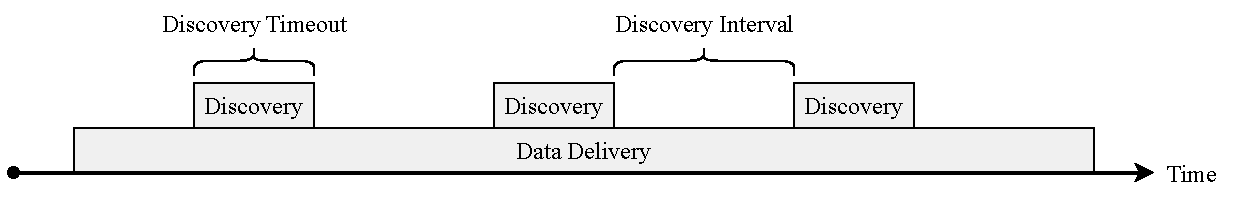
\includegraphics[width=.95\textwidth]{discovery_timers.pdf}
    \end{center}
    \caption{Sender: Discovery Timers}
    \label{fig:discovery_timers}
\end{figure}

\begin{figure}
    \begin{center}
        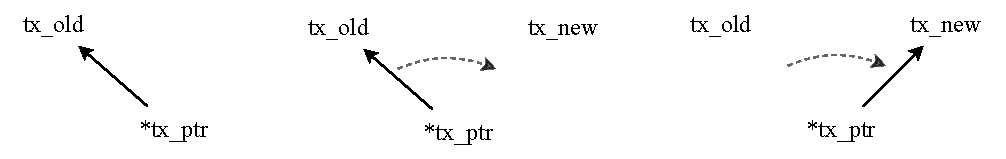
\includegraphics[width=.9\textwidth]{group_update.pdf}
    \end{center}
    \caption{Sender: Atomic update of the transmission group}
    \label{fig:group_update}
\end{figure}
% paragraph Discovery Thread (end)

\subsection{Grouping Algorithm} % (fold)
\label{sub:Grouping}
This section illustrates the receiver grouping algorithm, utilizing an exemplary
    topology tree depicted in \autoref{fig:mead_rcvr_grp}.
Initially, \hyperref[sec:Max 5]{Example 1} and \hyperref[sec:Max 10]{Example 2}
    outline the procedural steps of the algorithm for fundamental configurations.
\hyperref[sec:Max 10 Merge 1]{Example 3}, demonstrates the impact of the \textit{``Merge
    Range''} parameter (see \texttt{"--merge"} in \autoref{lst:send_help}).
\hyperref[sec:Max 12 Ok 7]{Example 4}, depicts the implication of the \textit{``OK Address
    List Length''} parameter (see \texttt{"--ok"} in \autoref{lst:send_help}).
\hyperref[sec:Max 10 Min Leaf 3]{Example 5} highlights the effect of the \textit{``Minimum
    Leaf Count''} parameter (see \texttt{"--min-leaves"} in \autoref{lst:send_help}).
A comprehensive description of all sender parameters is provided in \autoref{lst:send_help}.
Furthermore, \hyperref[alg:sender_grouping]{Algorithm 1} demonstrates the core grouping
    algorithm.

\subsubsection{Example 1:\quad Max. Address List Length: 5} % (fold)
\label{sec:Max 5}
In this example, we examine the topology depicted in \autoref{fig:mead_rcvr_grp},
    with a maximum address list length of five.
Initially, the sender $S$ conducts a \gls{dfs} to locate a router with unvisited
    leaves, yielding $R_2$ in our scenario.
Subsequently, a new \gls{mead} header is generated, encompassing $R_2$ along
    with its unvisited leaves, which are then marked as visited.
As the size of the address list is greater or equal to $\max-1$, no further
    addresses can be added, resulting in a header of \{$R_2$,$E_1$,$E_2$,$E_3$\}.
Another \gls{dfs} is initiated to identify the next router with unvisited leaves,
    resulting in $R_3$.
The procedure at $R_3$ mirrors that at $R_2$, resulting in
    \{$R_3$,$E_6$,$E_7$,$E_8$\}.
The subsequent \gls{dfs} yields $R_1$, and the procedure an identical procedure
    to that at $R_2$ is followed resulting in \{$R_1$,$E_4$,$E_5$\}.
As no unvisited leaves remain, the final grouping is \{$R_2$,$E_1$,$E_2$,$E_3$\},
    \{$R_3$,$E_6$,$E_7$,$E_8$\}, \{$R_2$,$E_1$,$E_2$,$E_3$\}.

\subsubsection{Example 2:\quad Max. Address List Length: 10} % (fold)
\label{sec:Max 10}
In this example, we analyze the topology depicted in \autoref{fig:mead_rcvr_grp},
    with a maximum address list length of ten.
The initial \gls{dfs} returns $R_2$.
Subsequently, a new \gls{mead} header is generated, encompassing $R_2$ along its
    unvisited leaves, which are then marked as visited.
The current state of the header is \{$R_2$,$E_1$,$E_2$,$E_3$\}.
If $R_2$ has a child router with unvisited leaves, we explore it.
However, given that $R_2$ has no child router, we ascend to $R_2$'s parent, $R_1$.
As the address list of the current header has sufficient space left for $R_1$
    and its unvisited leaves, they are appended, while the leaves are marked as
    visited.
The current state of the header is \{$R_2$,$E_1$,$E_2$,$E_3$,$R_1$,$E_4$,$E_5$\}.
If $R_1$ has a child router with unvisited leaves, we explore it, leading us to
    $R_3$.
As the address list of the current header cannot accommodate $R_3$ and its
    leaves, a new packet is created, resulting in \{$R_3$,$E_6$,$E_7$,$E_8$\}.
As no unvisited leaves remain, the final grouping is
    \{$R_2$,$E_1$,$E_2$,$E_3$,$R_1$,$E_4$,$E_5$\}, \{$R_3$,$E_6$,$E_7$,$E_8$\}.

\subsubsection{Example 3:\quad Max. Address List Length: 10, Merge Range: 1} % (fold)
\label{sec:Max 10 Merge 1}
In this instance, we examine the topology illustrated in \autoref{fig:mead_rcvr_grp},
    with a maximum address list length of ten and a merge range of one.
A merge range of one allows the sender $S$ to to merge leaves from distinct parent 
    routers under a common ancestor within a distance (\gls{mead} hops) of one.
The initial \gls{dfs} returns $R_2$.
Subsequently, a new \gls{mead} header is generated, encompassing $R_2$ along its
    unvisited leaves, which are then marked as visited.
The current state of the header is \{$R_2$,$E_1$,$E_2$,$E_3$\}.
If $R_2$ has a child router with unvisited leaves, we explore it.
However, given that $R_2$ has no child router, we ascend to $R_2$'s parent, $R_1$.
As the address list of the current header has sufficient space left for $R_1$'s
    unvisited leaves, they are merged, while the leaves are marked as visited.
The current state of the header is \{$R_2$,$E_1$,$E_2$,$E_3$,$E_4$,$E_5$\}.
If the currently considered router ($R_1$) is closer to the sender $S$ than the
    router in the address list ($R_2$), we set $R_1$ as the designated
    router, resulting in \{$R_1$,$E_1$,$E_2$,$E_3$,$E_4$,$E_5$\}.
If $R_1$ has a child router with unvisited leaves, we explore it, leading us to
    $R_3$.
As the address list of the current header has sufficient space left for $R_3$'s
    unvisited leaves, they are merged, while the leaves are marked as visited.
The current state of the header is
    \{$R_1$,$E_1$,$E_2$,$E_3$,$E_4$,$E_5$,$E_6$,$E_7$,$E_8$\}.
Since the currently considered router ($R_3$) is not closer to the sender $S$ than
    the router in the address list ($R_1$), there is no need to update the
    designated router in the address list.
As no unvisited leaves remain, the final grouping is
    \{$R_1$,$E_1$,$E_2$,$E_3$,$E_4$,$E_5$,$E_6$,$E_7$,$E_8$\}.

\subsubsection{Example 4:\quad Max. Address List Length: 12, OK Addres List Length: 7}
\label{sec:Max 12 Ok 7}
In this example, we examine the topology demonstrated in \autoref{fig:mead_rcvr_grp},
    with a maximum address list length of twelve and a ``OK'' address list length
    of seven.
A ``OK'' address list length of seven allows the sender $S$ to prematurely finish
    a packet, if it contains an equal or greater number of addresses than seven.
The initial \gls{dfs} returns $R_2$.
Subsequently, a new \gls{mead} header is generated, encompassing $R_2$ along its
    unvisited leaves, which are then marked as visited.
The current state of the header is \{$R_2$,$E_1$,$E_2$,$E_3$\}.
If $R_2$ has a child router with unvisited leaves, we explore it.
However, given that $R_2$ has no child router, we ascend to $R_2$'s parent, $R_1$.
As the address list of the current header has sufficient space left for $R_1$
    and its unvisited leaves, they are appended, while the leaves are marked as
    visited.
The current state of the header is \{$R_2$,$E_1$,$E_2$,$E_3$,$R_1$,$E_4$,$E_5$\}.
As the length of the address list is greater or equal to ``OK'' address list
    length, no further addresses are added to the list, even though $R_3$ and
    its unvistited leaves could be acommendated.
Another \gls{dfs} is initiated to identify the next router with unvisited leaves,
    resulting in $R_3$.
The procedure at $R_3$ mirrors that at $R_2$, resulting in
    \{$R_3$,$E_6$,$E_7$,$E_8$\}.
As no unvisited leaves remain, the final grouping is
    \{$R_2$,$E_1$,$E_2$,$E_3$,$R_1$,$E_4$,$E_5$\}, \{$R_3$,$E_6$,$E_7$,$E_8$\}.

\subsubsection{Example 5:\quad Max. Address List Length: 10, Min. Leaf Count: 3}
\label{sec:Max 10 Min Leaf 3}
In this instance, we examine the topology illustrated in \autoref{fig:mead_rcvr_grp},
    with a maximum address list length of ten and a merge range of one.
With a minimum leaf count of three the sender $S$ marks all leaves of routers with
    less than three leaves for unicast delivery.
The initial \gls{dfs} returns $R_2$.
Subsequently, a new \gls{mead} header is generated, encompassing $R_2$ along its
    unvisited leaves, which are then marked as visited.
The current state of the header is \{$R_2$,$E_1$,$E_2$,$E_3$\}.
If $R_2$ has a child router with unvisited leaves, we explore it.
However, given that $R_2$ has no child router, we ascend to $R_2$'s parent, $R_1$.
As $R_1$ has less than three leaves, its leaves are appended to the unicast
    delivery list, and marked as delivered.
If $R_1$ has a child router with unvisited leaves, we explore it, leading us to
    $R_3$.
As the address list of the current header has sufficient space left for $R_3$'s
    unvisited leaves, they are merged, while the leaves are marked as visited.
The current state of the header is
    \{$R_2$,$E_1$,$E_2$,$E_3$,$R_3$,$E_6$,$E_7$,$E_8$\}.
As no unvisited leaves remain, the final grouping is
    \textit{MEADcast}: \{\{$R_2$,$E_1$,$E_2$,$E_3$,$R_3$,$E_6$,$E_7$,$E_8$\}\},
    \textit{Unicast}: \{$E_6$,$E_7$\}.
% basic grouping algorithm:
%   - search start (dfs)
%   - while free leaf:
%       - if cgs > max
%           - finish group
%           - goto search start
%       - if cgs >= max - 1
%           - add router to group
%           - recursively update parent counters
%           - finish group
%           - goto search start
%       - if cgs < max
%           - add router to group
%   - while free child:
%       - get free router child
%       - goto start
%   - if parent
%       - backpropagate
%       - if parent is root
%           - finish group
%       - goto start
    %
% effect of merge and split parameter

% hash table:
%   - stores pointer to node (router or leaf)
%   - used to quickly find ip
% *rcvr:
%   - linked list of all receivers
%   - used to quickly get all receivers
% tree:
%   - consists of nodes (router or leaf)
%   - sender is root
%   - used to group endpoints

% Grouping:
% 1) Reduce tree
%   - Remove routers with less leaves or routers than X. Childs are adopted by parent
% 2) Grouping
%   - search start (dfs)
% paragraph Grouping (end)

% Startup
% - Create TUN dev (set MTU, set Route)
% - txg only struct shared between threads
% - Implemented in C (efficiency & comparable to other protocols)
% - TUN
% - Automatically set route & MTU
% - Judy Array to quickly find IPs
% - Tree for grouping
% - grouping algorithm
% section Sender (end)

\begin{figure}
\centering
\begin{forest}
    for tree={grow=south, circle, draw, align=center, font=\footnotesize, l sep=7ex},
        where level=0{minimum size=2.3em, l sep-=3.5ex}{},
        where level=1{
            s sep+=10pt
        }{},
        % where level=4{l sep-=40}{},
        % where n children=0{tier=bottom}{},
        where n children=0{minimum size=2.3em}{},
    [$S$
        [$R_1$
            [$R_2$ [$E_1$][$E_2$][$E_3$]]
            [$E_4$][$E_5$]
            [$R_3$ [$E_6$][$E_7$][$E_8$]]
            ]
        ]
    ]
\end{forest}
    \caption[MEADcast network topology tree]{\gls{mead} network topology tree.
    $S$ represents the sender, $R_i$ \gls{mead} routers, and $E_j$ group members.}
\label{fig:mead_rcvr_grp}
\end{figure}

\begin{algorithm}
    \caption{Sender: grouping algorithm}\label{alg:sender_grouping}
    \hspace*{\algorithmicindent} \textbf{Input:} Router ($s$) to start grouping at\\
    \hspace*{\algorithmicindent} \textbf{Output:} \texttt{tx\_group} structure\\
\begin{algorithmic}[1]
\State $group\gets NULL$\Comment{\texttt{tx\_group} structure}
\State $m\gets 0$
\State $n\gets 0$
\State $r\gets \text{getStart($s$)}$
\Comment{Gets next router based on depth-first search}
\While{$r$}
\Label \texttt{start:}
    \While{$r.freeLeaves > 0$}
        \State $m\gets n + r.freeLeaves + 1$
        \If{$m > max$}
            \State \textbf{go to} \texttt{start}
        \ElsIf{$m \geq max - 1$}
            \State addRouterToGroup($r$)
            \Comment{Update bitmaps and address list}
            \State recursiveBackpropergate($r$)
            \Comment{Update leaf and child count of all anchestors}
            \State \textbf{go to} \texttt{next}
        \ElsIf{$m < max$}
            \State addRouterToGroup($r$)
            \State \textbf{break}
        \EndIf
    \EndWhile
    \While{$r.freeChild > 0$}
        \State $c\gets \text{getFreeRouter($r$)}$
        \If{c}
            \State $r\gets \text{getRouter($c$)}$
            \State \textbf{go to} \texttt{start}
        \EndIf
    \EndWhile
    \If{$r.node.parent$}
        \State backPropagate($r$)
        \Comment{Update parent leaf and child count}
        \State $r\gets \text{getRouter($r.node.parent$)}$
        \If{\textbf{not}\ r.node.parent}
            \Comment{If parent is root finish group}
            \State \textbf{go to} \texttt{next}
        \EndIf

        \State \textbf{go to} \texttt{start}
    \EndIf
\Label \texttt{next:}
    \State finishGroup()
    \Comment{Adds MEADcast header to \texttt{group.mdc} list}
    \State $r\gets \text{getStart($r$)}$
\EndWhile
    \State addRemainingLeaves($s$)
    \Comment Adds the remaining leaves to \texttt{group.uni} list 
    \State \Return $group$
\end{algorithmic}
\end{algorithm}


\section{Experiment} % (fold)
\label{sec:Experiment}
This section illustrates the implementation of the experiment.
Initially, \autoref{sub:Network Topology} depicts the network topology and
    the selected designs for each use case.
Subsequently, \autoref{sub:Technical Infrastructure} delves into the deployment
    process of our virtual testbed.
Finally, \autoref{sub:Conduction} provides insights into the conduction
    of each use case.

\subsection{Network topology} % (fold)
\label{sub:Network Topology}
This section provides detailed insights into the designed experiment topology.
Furthermore, it highlights the specific selection of sender, receivers, and
    routers for each use case.

\subsubsection{Topology} % (fold)
\label{sec:Topology}
The architecture of our testbed aligns with the in \autoref{sub:Topology}
    formulated requirements, achieved through the implementation of the
    hierarchical three-layer model.

% less clinical / more variety so sometimes two routers on access layer
The testbed comprises 205 nodes consisting of 40 routers and 165 end devices.
The network is divided into four domains, each potentially representing distinct
    buildings on a university campus.
All four domains encompass seven to nine client networks, accommodating five
    end devices each.
The access layer of each domain comprises up to seven routers (3-digit router IDs
    in \autoref{fig:topology}).
Since this thesis evaluates a transport protocol, we waive the application of
    switches on the access layer, deploying solely layer 3 devices.
The distribution layer of each domain encompasses two to three interconnected routers
    (2-digit router IDs), aggregating the access layers within its respective
    domain and facilitating the connection to the core layer.
The testbed's core consists of routers routers (1-digit router IDs) interconnecting
    the four network domains.
Additionally, the backbone possesses a high connectivity, ensuring both high
    availability and redundancy.
To reduce management and operational overhead, the testbed incorporates fewer
    redundant links from the access to the distribution layer and from the
    distribution to the core layer compared to the recommendations provided by
    Cisco and Huawei \cite{cisco_design_guide,huawei_campus_net}.
This trade-off is considered acceptable, as this thesis does not delve into the
    details of the availability and fault tolerance of the network
    architecture.
Additionally, router and link failures are artificially induced in any case.

The chosen architecture represents a realistic medium-sized network topology.
The application of the hierarchical three-layer model ensures the required
    flexibility of the testbed.
Various placements of senders, receivers, and routers are possible, allowing
    experiments with a receiver distribution ranging from high clustering
    within a single domain to a uniform spread across all four network domains.
Moreover, the availability of alternative routes facilitates the representation
    of dynamic network environments, encompassing scenarios such as deliberate
    routing changes or router and link outages.

\begin{figure}
    \begin{center}
        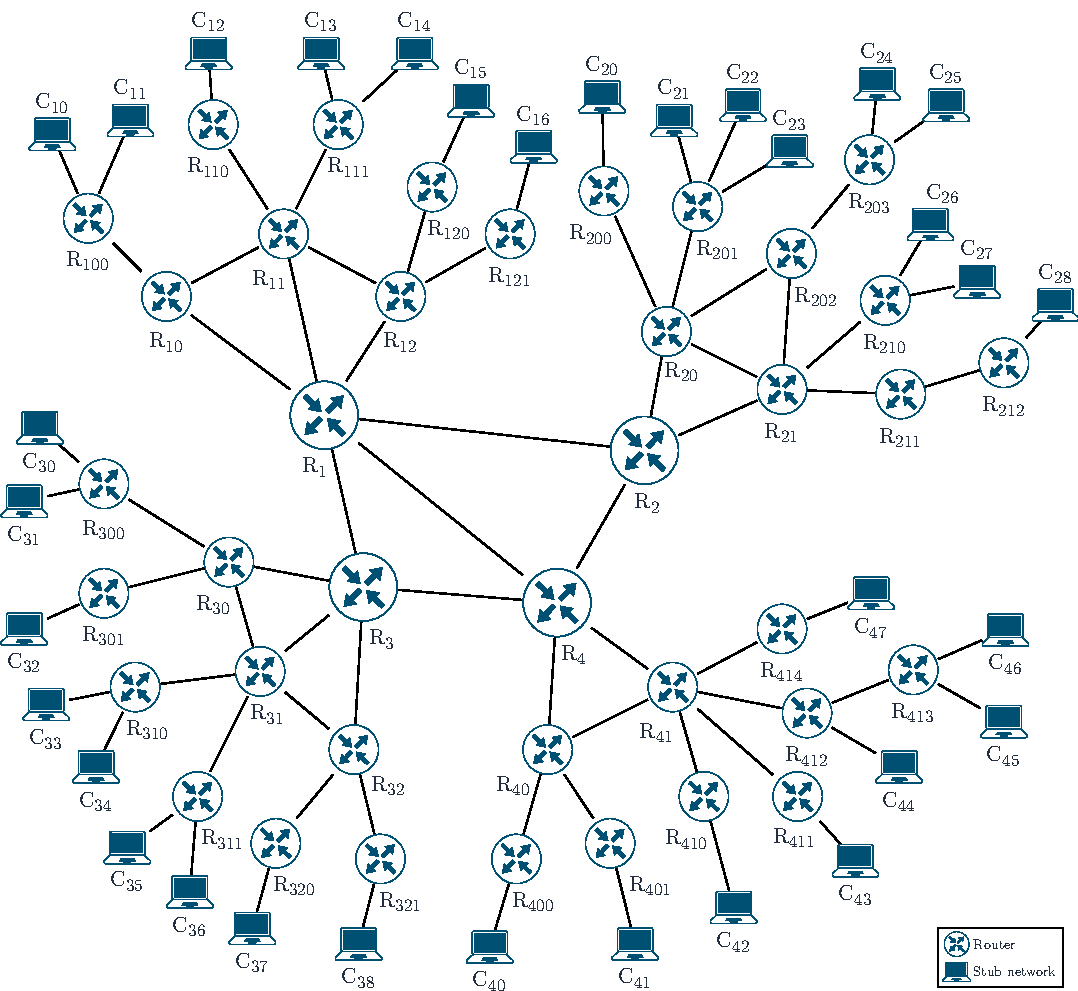
\includegraphics[width=.65\textwidth]{testbed_topology.pdf}
    \end{center}
    \caption{Testbed Topology}
    \label{fig:topology}
\end{figure}

% subsubsection Topology (end)



\subsubsection{UC1: Live Stream} % (fold)
\label{par:impl UC1: Live Stream}
In accordance with the requirements outlined for \uci{} in
    \autoref{par:EX1: Live Stream}, \autoref{fig:exp_live_stream} illustrates
    the chosen topology, which comprises up to 96 nodes, consisting of a
    maximum of 70 receivers (with a maximum of five per client network) and 26
    routers.
% The topology for UC1 is depicted in \autoref{fig:exp_live_stream}, consisting of
%     up to 96 nodes, comprising up to 70 receivers (max. 5 per client network) and
%     26 routers.
The configuration encompasses four network domains each representing a building
    on a campus or even an entire location.
Client $C_{3001}$ is designated as the sender.
Areas within client networks $C_{21}$-$C_{23}$, $C_{35}$-$C_{36}$, and
    $C_{41}$-$C_{46}$ exhibit high receiver clustering, while networks
    $C_{11}$, $C_{14}$, $C_{16}$, $C_{28}$, and $C_{38}$ demonstrate low
    receiver density.
The selection of client networks encompasses varying distances between sender
    $C_{3001}$ and receivers, ranging from four hops for $C_{35}$ and $C_{36}$
    to eight hops for $C_{28}$.

The chosen topology aligns with the requirements formulated in
    \autoref{par:EX1: Live Stream} and facilitates the measurement of
    \gls{mead}'s performance for mid to large-sized groups, incorporating a
    mixture of highly clustered and isolated nodes.
This highlights the protocol's potential in scenarios of heterogeneous receiver
    distributions.

\begin{figure}
    \begin{center}
        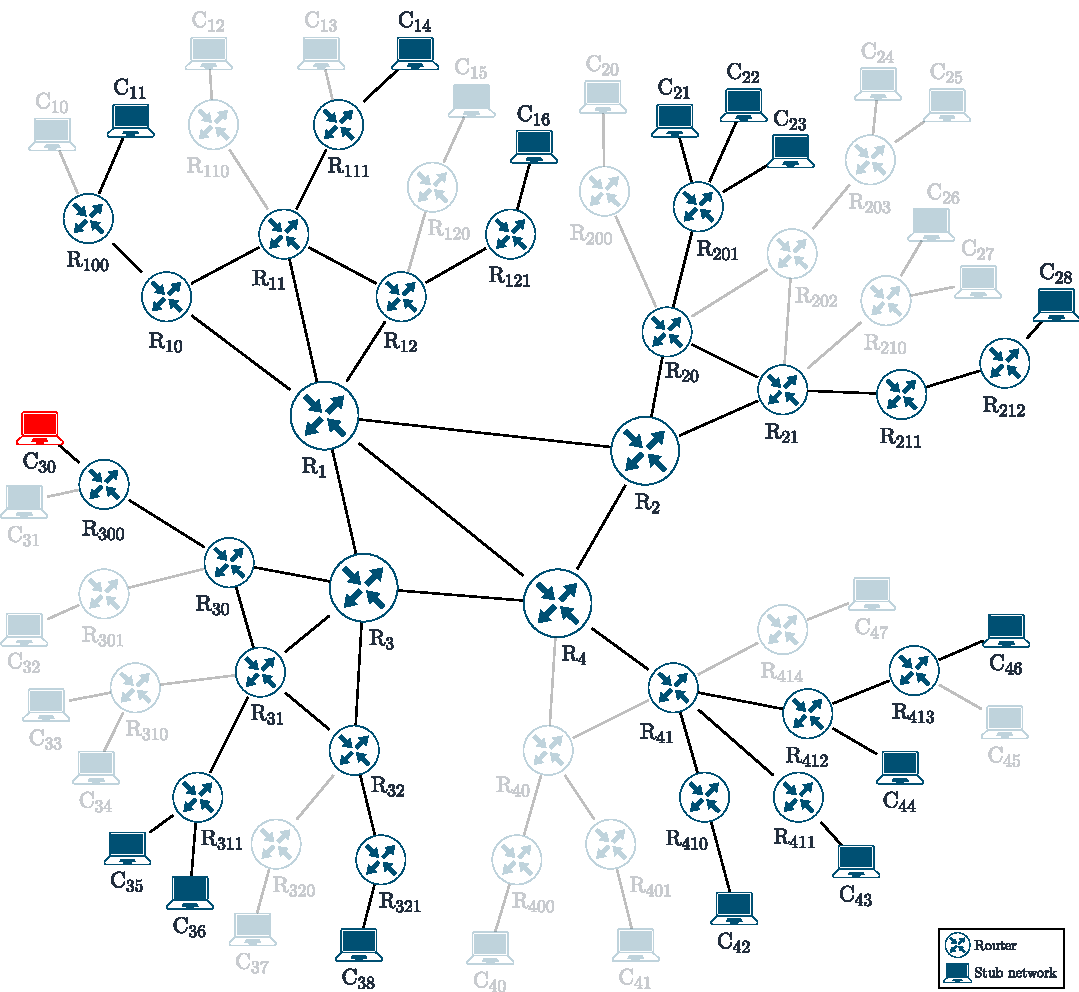
\includegraphics[width=.7\textwidth]{exp_live_stream.pdf}
    \end{center}
    \caption[UC1: Live Stream]{\nuci{} ($C_{3001}$ \textit{is sender})}
    \label{fig:exp_live_stream}
\end{figure}
% subsubsection UC1 Live Stream (end)


\subsubsection{UC2: File transfer} % (fold)
\label{par:implEX2: File transfer}
In accordance with the requirements provided for \ucii{} in
    \autoref{par:EX2: File Transfer}, \autoref{fig:exp_file_transfer}
    illustrates the chosen topology, consisting of up to 58 nodes, comprising
    45 receivers (with a maximum of five per client network) and 13 routers.
The node selection encompasses the entire network domain three, representing
    either a server network or even an entire data center, with the sender
    $C_{4001}$ serving as the package source mirror. 
All client networks ($C_{30}$-$C_{38}$) are located within one highly
    clustered area.
Furthermore, we have the flexibility to adjust the number of receivers by
    scaling the number of active nodes within a client network within a range
    of one to five.

The chosen topology aligns with the requirements outlined in
    \autoref{par:EX2: File Transfer} and facilitates the evaluation of
    \gls{mead}'s performance for mid to large-sized groups of highly clustered
    nodes, demonstrating the protocol's potential in scenarios with ideal
    conditions.

\begin{figure}
    \begin{center}
        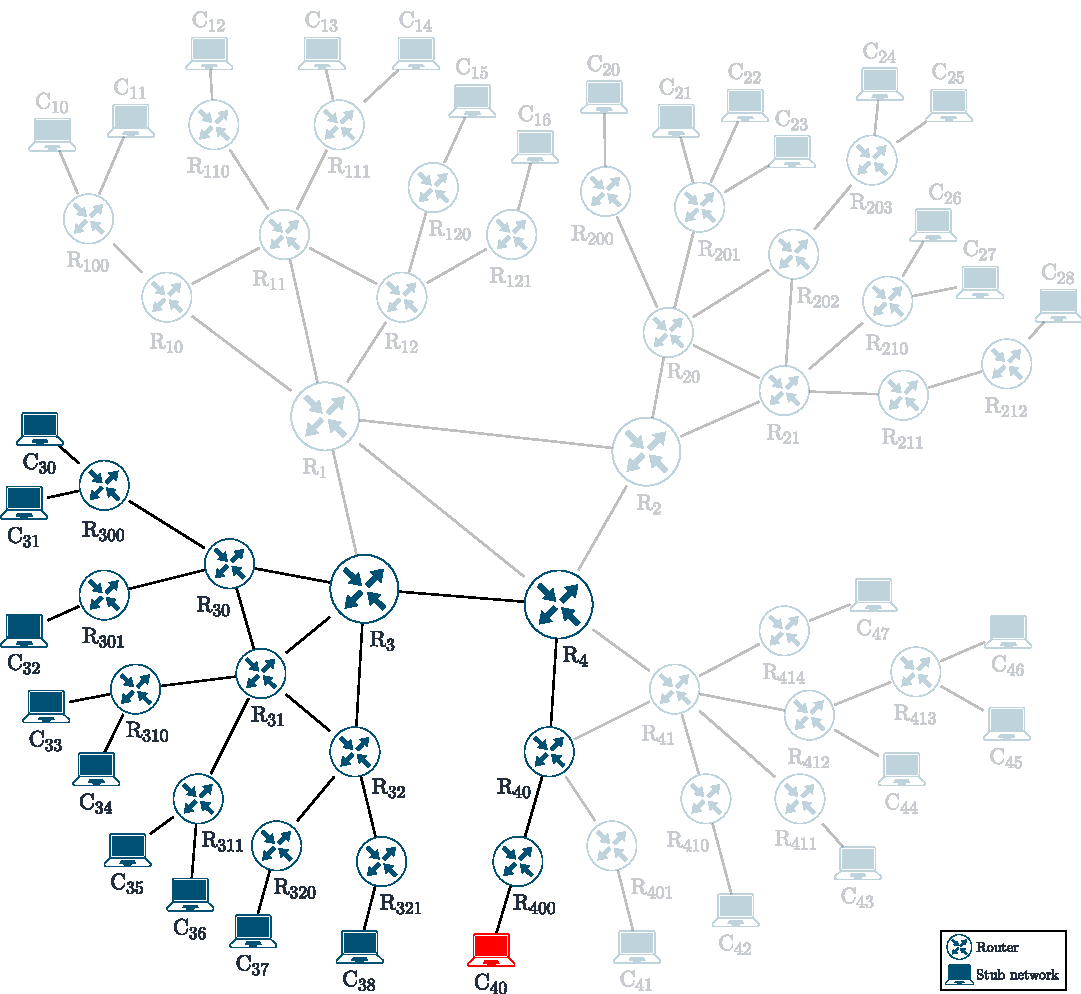
\includegraphics[width=.7\textwidth]{exp_file_transfer.pdf}
    \end{center}
    \caption[UC2: File Transfer]{\nucii{} ($C_{4001}$ \textit{is sender})}
    \label{fig:exp_file_transfer}
\end{figure}

\subsubsection{UC3: P2P Video conference} % (fold)
\label{par:impl EX3 Video conference}
In accordance with the requirements formulated for \uciii{} in
    \autoref{par:EX3 Video conference}, \autoref{fig:exp_video_conference}
    depicts the chosen topology, including a total of up to 78 nodes, comprising
    60 clients (with a maximum of five per client network) and 18 routers.
However, since this use case aims to assess \gls{mead}'s suitability for small
    to medium-sized \gls{p2p} conferences, the number of clients is typically
    lower.
The topology features local clustering in the area of $C_{33}$-$C_{36}$
    and $C_{21}$-$C_{25}$, representing sub-teams in different office locations.
Conversely, $C_{12}$, $C_{40}$, and $C_{46}$ exhibit a low receiver density
    representing customers or service providers in remote areas.
The selection of client networks encompasses varying distances between clients,
    ranging from one hop within local clusters such as between $C_{33}$ and
    $C_{34}$, up to eight hops between $C_{25}$ and $C_{46}$.
Since this use case focuses on \gls{p2p} communication, all clients transmit
    and receive traffic.

The chosen topology aligns with the requirements stated in
    \autoref{par:EX3 Video conference} and facilitates the investigation of
    \gls{mead}'s suitability for \gls{p2p} communication and whether the
    protocol can bridge the asymmetric access link bandwidth.
Moreover, the topology enables the examination of the effect of high \gls{mead}
    traffic volume on \gls{mead} routers.

\begin{figure}
    \begin{center}
        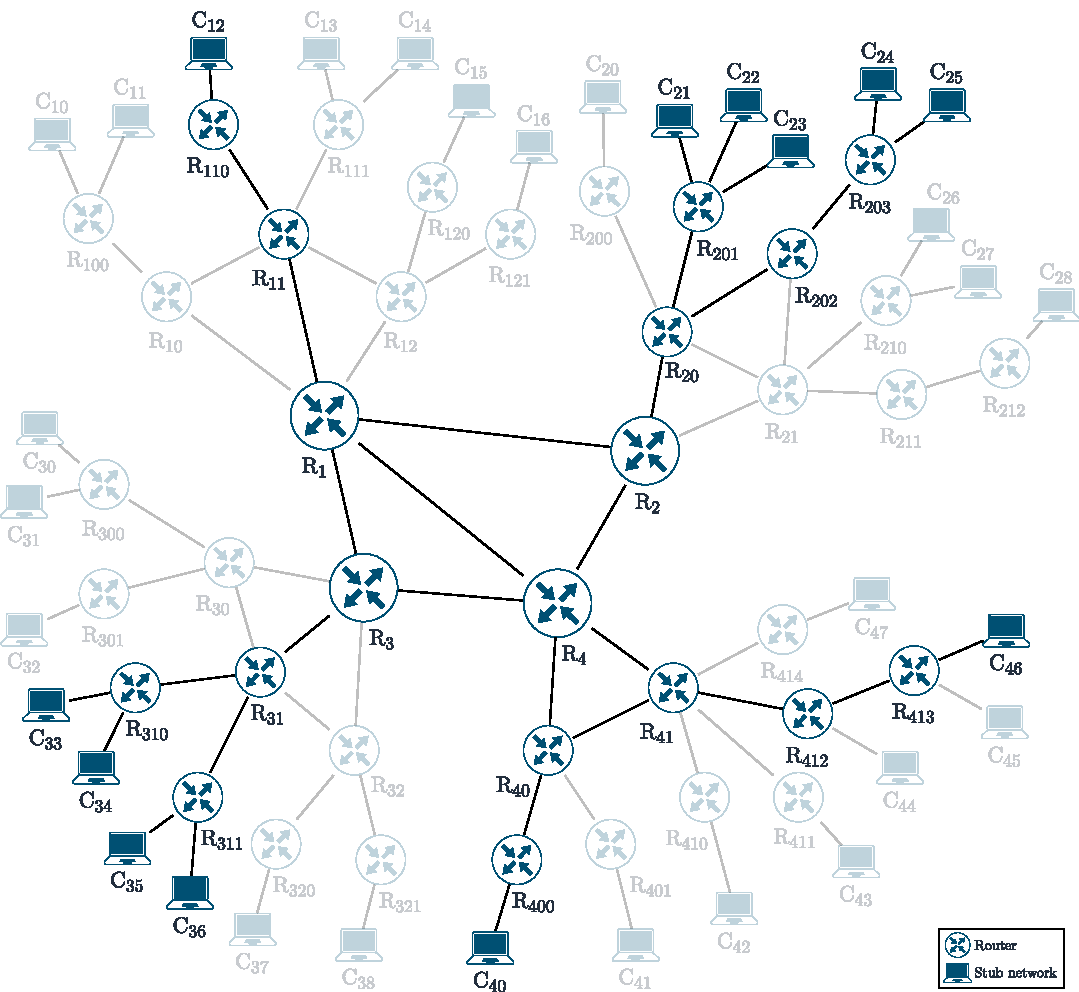
\includegraphics[width=.7\textwidth]{exp_video_conference.pdf}
    \end{center}
    \caption[UC3: P2P Video Conference]{\nuciii{} (\textit{all members are senders})}
    \label{fig:exp_video_conference}
\end{figure}

\subsubsection{UC4: Online Gaming} % (fold)
\label{par:EX4 Online Gaming}
In accordance with the requirements outlined for \uciv{} in
    \autoref{par:EX4 Online game}, \autoref{fig:exp_online_gaming}
    illustrates the chosen topology, comprising up to 72 nodes, including
    45 receivers (with a maximum of five per client network) and 27 routers.
However, since this use case aims to assess \gls{mead}'s suitability for small
    to medium-sized groups, the number of clients is typically lower.
The design features an evenly spread distribution of client networks with a low
    receiver density.
No router is directly connected to more than one client network.
Client $C_{4501}$ is designated as the sender.
The selection of client networks encompasses varying distances between sender
    and receivers, ranging from four hops for $C_{43}$ up to eight hops for
    $C_{24}$ and $C_{28}$.

The chosen topology design aligns with the requirements provided in
    \autoref{par:EX4 Online game} and facilitates the evaluation of \gls{mead}'s
    implication on latency and jitter.
Moreover, the topology enables the investigation of \gls{mead}'s performance in
    scenarios with suboptimal conditions, particularly with a high receiver
    distribution.

\begin{figure}
    \begin{center}
        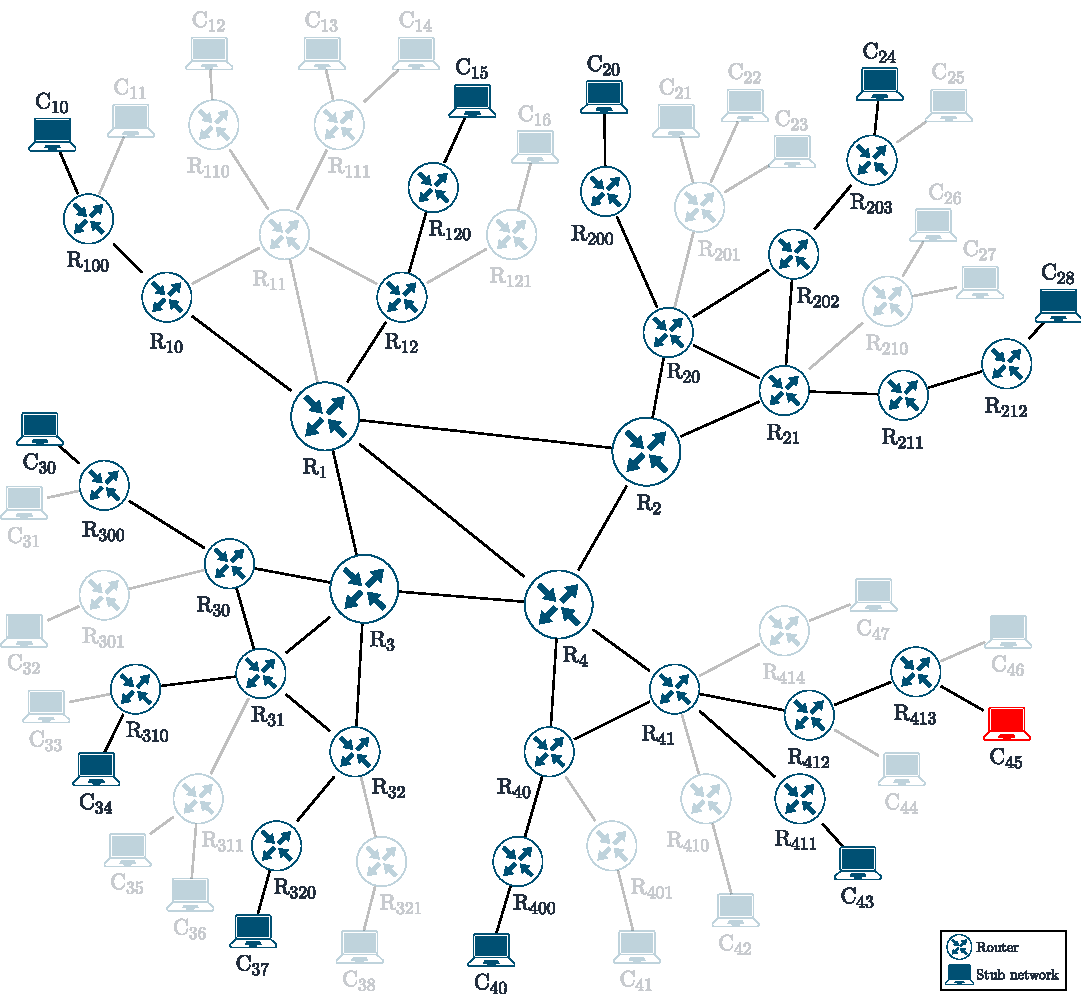
\includegraphics[width=.7\textwidth]{exp_online_gaming.pdf}
    \end{center}
    \caption[UC4: Online Gaming]{\nuciv{} ($C_{45}$ \textit{is sender})}
    \label{fig:exp_online_gaming}
\end{figure}
% subsection Testbed (end)


\subsection{Technical Infrastructure} % (fold)
\label{sub:Technical Infrastructure}
%%% Facts
% Hardware Resources
% Debian Version
% KVM
% para virtualized Net IO Dev
% One backing file, and vm disk only tracking differences.
% Debian No-Cloud Image Version for clients
% Direct Kernel boot for router
% VM resources
Given the impracticality of creating a physical testbed, we have opted for a 
    virtual environment using \gls{kvm}.
The testbed comprises \glspl{vm} connected by virtual networks.
The hypervisor, based on Debian 11.3, is equipped with 4 CPUs, 8 threads, 32 GB
    memory, and 120 GB of storage capacity.

Each \gls{vm} is configured with 1 vCPU, 256 MB, and 8 GB of storage.
To optimize resource utilization, we employ the para-virtualized ``virtio''
    network adapter for the \glspl{vm}.
We utilize two types of \glspl{vm}: clients and routers, both based on a Debian
    11 no-cloud image.
No-cloud images streamline the setup process by bypassing the need for \gls{os}
    installation.
Additionally, direct Kernel boot is facilitated for the router, enabling swift
    kernel exchange by simply replacing the Kernel image file on the
    hypervisor.

% template images
During the build process, a router and a client template image are created.
These serve as \textit{``Qemu''} backing files for the \gls{vm} images,
    ensuring that \glspl{vm} only have to monitor changes compared to the
    backing template, reducing storage usage and build time significantly.

%%% How created
% python script virsh util
% from json file describing topo
% frr for routing, had to change repo bc ospf6 was missing
% ospf6 and Pim as routing protocols
% ospf domains
% chrony ptp for time sync, had to add kernel boot arg to make it work
% each vm a IPv6 only MGM if and other interfaces IPv6 only
% IP addressing concept
% each transit link neads a non link local address to make MEADcast work
% command to build topo
Automating the build process is a Python script provided in the digital
    appendix, with the command to construct our topology shown in
    \autoref{lst:cmd_mk_topo_start}.
The script presents a wrapper around tools such as ``\textit{virsh}'',
    ``\textit{libguestfs-tools}'', and ``\textit{qemu-img}''.
It accepts several input parameters, including template configuration files
    for the virtual network generation, ``\textit{chrony}'' (time
    synchronization), and ``\textit{frr}'' (routing).
Additionally, the script requires a Kernel image for the router and a
    configuration file describing the network topology.
\autoref{lst:topo_cfg_format} demonstrates an exemplary topology definition,
    resulting in the topology shown in \autoref{fig:ex_topo}.
The  \texttt{"stub"} key from the topology configuration contains a list of
    objects describing a stub network, its number of clients, the upstream
    router, and the OSPF area.
The \texttt{"trans"} key includes a list of objects comprising a tuple of two
    router IDs and OSPF area.
The routers are interconnected according to this list.
The \texttt{"area\_boundary"} key consists of a list of objects representing
    the OSPF boundaries, by router ID, OSPF area ID, and the network mask
    of the published summarizing route.

The IP naming scheme for client machines follows the format
    \texttt{"fd14::<AREA ID>:<ROUTER ID>:<CLIENT ID>"}.
Additionally, each \gls{vm} is attached to an IPv4 management network.
The clients utilize static routing, with a default IPv4 route on the management
    interface and a ``fd14::/16'' route on the upstream interface.

% Time sync
For accurate measurement of latency and jitter, synchronized clocks among the
    \glspl{vm} are imperative.
While \gls{ntp} is a common solution for time synchronization, Linux provides
    an alternative mechanism that does not require an \gls{ntp} server or the 
    network stack at all.
Instead, the host injects para-virtualized \gls{ptp} devices into the guests
    facilitating highly accurate time synchronization.
Apart from loading the \texttt{"kvm\_ptp"} Kernel module and configuring
    \textit{``chrony''} as usual, setting the clock source on the host via
    Kernel command line parameters to \texttt{"clocksource=tsc"} was necessary.

% Router, routing protocol,
The router operates on our custom \gls{mead} Kernel version 6.5.2.
\textit{``Frr''} facilitates the routing stack, which supports a variety of
    routing protocols such as BGP, OSPF, RIP, and PIM \cite{frr_doc}.
OSPF is utilized as the IP Unicast routing protocol and PIM for IP Multicast
    routing.
Beyond the standard setup of \textit{``frr''}, manual alteration of the package
    manager source to \url{https://deb.frrouting.org/} was necessary, as the
    package from the default source misses the IPv6 PIM daemon.
It is noteworthy while OSPF mandates routers to possess only a link-local
    address, the \gls{mead} discovery phase necessitates each router to have at
    least one global IPv6 address.

\begin{figure}
    \begin{center}
        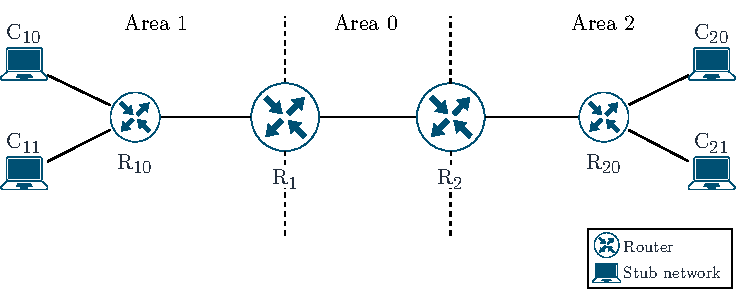
\includegraphics[width=0.75\textwidth]{topo_format.pdf}
    \end{center}
    \caption[Example topology]{
        Example topology generated from the configuration file shown in
        \autoref{lst:topo_cfg_format}.
    }
    \label{fig:ex_topo}
\end{figure}

% subsection Technical Infrastructure (end)
% section Experiment (end)

\subsection{Conduction} % (fold)
\label{sub:Conduction}
% How conducted
% How evaluated

% More than 180 experiments, repeated multiple times to ensure validity
% 120 measurements EX1, 50 EX2, 10 EX3
We conducted over 180 measurements across three distinct use cases (UC1-3),
    repeating each measurement multiple times to ensure the validity and
    reliability of the collected data.
Specifically, we conducted more than 120 measurements for \uci{}, 50 for
    \ucii{}, and 10 for \uciii{}.

Each \textit{use case} is delineated by its compilation of routers, transit and
    stub networks, and specific application characteristics, including
    communication and traffic pattern.
An \textit{experiment} entails executing a series of measurements for a given
    use case, featuring a specific number of clients and data volume.
This series comprises measurements for IP Unicast, IP Multicast, and various 
    \gls{mead} configurations.
A \gls{mead} configuration is composed of the sender parameterization and the 
    network support level.
For instance, \autoref{tab:usecase_experiment_measurement} provides an excerpt
    of two experiments conducted within \nuci{}.

\begin{table}
\centering
\begin{tabular}{@{}ccccccccccc@{}}
\toprule
& & \multicolumn{3}{c}{\textbf{Experiment}} & \multicolumn{6}{c}{\textbf{MEADcast}} \\
\cmidrule(lr){3-5}\cmidrule(lr){6-11}
& &
\multicolumn{2}{c}{Clients}
& & &
\multicolumn{3}{c}{Discovery} &
\multicolumn{2}{c}{Grouping} \\
\cmidrule(lr){3-4}\cmidrule(lr){7-9}\cmidrule(lr){10-11}

\textbf{\makecell[c]{Use\\case}} &
    Proto.   &
    Tot.      &
    \makecell[c]{per\\Router} &
    \makecell[c]{Vol.\\\itshape (MB/s)}       &
    \makecell[c]{Net.\\Supp.}       &
    \makecell[c]{Dly\\\itshape (s)}    &
    \makecell[c]{Intvl\\\itshape (s)}     &
    \makecell[c]{T. out\\\itshape (s)}    &
    \makecell[c]{Max.\\size}       &
    \makecell[c]{Merge\\range}      \\ \midrule
Stream   & Uni      & 14        & 1         & 1      & -      & -      & -         & -         & -               & -          \\
Stream   & Multi    & 14        & 1         & 1      & -      & -      & -         & -         & -               & -          \\
Stream   & Mead     & 14        & 1         & 1      & 100\%  & 0      & 0         & 0         & 10              & 0          \\
Stream   & Mead     & 14        & 1         & 1      & 100\%  & 0      & 5         & 2         & 10              & 0          \\
\vdots   & \vdots   & \vdots    & \vdots    & \vdots & \vdots & \vdots & \vdots    & \vdots    & \vdots          & \vdots \\[3pt]
Stream   & Mead     & 14        & 1         & 1      & 100\%  & 0      & 0         & 0         & 10              & 2          \\
Stream   & Mead     & 14        & 1         & 1      & L1     & 0      & 0         & 0         & 20              & 0          \\ \midrule
Stream   & Uni      & 28        & 2         & 2.5    & -      & -      & -         & -         & -               & -          \\
Stream   & Multi    & 28        & 2         & 2.5    & -      & -      & -         & -         & -               & -          \\
Stream   & Mead     & 28        & 2         & 2.5    & 100\%  & 0      & 0         & 0         & 10              & 0          \\
Stream   & Mead     & 28        & 2         & 2.5    & 100\%  & 0      & 5         & 2         & 10              & 0          \\
\vdots   & \vdots   & \vdots    & \vdots    & \vdots & \vdots & \vdots & \vdots    & \vdots    & \vdots          & \vdots \\[3pt]
Stream   & Mead     & 28        & 2         & 2.5    & 100\%  & 0      & 0         & 0         & 10              & 2          \\
Stream   & Mead     & 28        & 2         & 2.5    & L1     & 0      & 0         & 0         & 20              & 0          \\
\bottomrule
\end{tabular}
\caption[Use case, experiments and measurements]{
    Use case, experiments and measurements.
    Excerpt of two experiments comprising multiple measurements conducted
    within \nuci{}.
}
\label{tab:usecase_experiment_measurement}
\end{table}

\paragraph{Measurment} % (fold)
\label{par:Measurment}

% Always measured all links. Used ifstat on host (bc each network is just a bridge)
We utilized \textit{``Iperf2''} for the data transmission and to collect
    performance metrics including sender and receiver bandwidth utilization,
    latency, jitter, and packet loss.
The usage of \textit{``Iperf3''} was not feasible due to the necessity of an
    initial \gls{tcp} handshake.

% Used Iperf to measure tx/rx bw utilization, latency, jitter, packet loss
To measure the total network bandwidth utilization, we monitored all links
    within the use case.
As the experiments were conducted in a virtual environment, we simply needed to
    measure the receive and transmission bandwidth of each virtual network,
    which is essentially a network bridge on the host system.
For this purpose, we utilized \textit{``ifstat''}.
To measure CPU and memory utilization, we employed a tool called \textit{``sar''}.
However, during the majority of our measurements, resource utilization peaked,
    hindering our ability to obtain meaningful results.
% paragraph Measurment (end)

\paragraph{RX/TX} % (fold)
\label{par:RX/TX}
% Uni (1:n):
%   - rx: ssh into all machines, start Iperf server and detach from it
%   - tx: ssh into sender and start one Iperf instance per receiver via gnu parallel
To conduct IP Unicast measurements for \uci{} and \ucii{} we connected to all
    receivers using GNU parallel and SSH, initiated Iperf in server mode and
    detached from the process (see \autoref{lst:uni_start_cmd}).
On the sender we initiated one instance of \textit{``Iperf''} per receiver using GNU
    parallel.

% Multicast:
%   - rx: same as Unicast (but listen on Multicast address)
%   - tx: start Iperf client on sender with Multicast address
For the IP Multicast measurements, the procedure on the receiver side is
    identical to IP Unicast, except that Iperf listens on a IPv6 Multicast
    address (see \autoref{lst:multi_start_cmd}).
On the sender side, one instance of Iperf is started to transmit traffic
    towards all multicast listeners.

% \gls{mead}:
%   - rx: same as Unicast
%   - tx: start MEADcast sender, and send IPerf into TUN dev
To measure \gls{mead}, the procedure on the receiver side is identical to IP
    Unicast (see \autoref{lst:mead_start_cmd}).
On the sender we started the \gls{mead} sender implementation and configured
    Iperf to send its traffic into the TUN device, as shown in
    \autoref{fig:tun_dev}.
It is noteworthy, that we initiated the Iperf client (our sender) with the
    \texttt{"--no-udp-fin"} flag to prevent the Iperf server (our receivers)
    from sending a final report to the client, potentially falsifying our
    bandwidth measurements.

% Uni (m:n):
%   - rx: same
%   - tx: ssh into each client and do the same as 1:n
To conduct IP Unicast measurements for \uciii{} (\gls{p2p}), we employed one
    instance of Iperf in server mode on each client ($n$), along with $n-1$
    instances of Iperf in client mode, sending traffic to each other.
% Multicast (m:n)
%   - not possible, bc Iperf requires receiver to bind to Unicast host to listen to
%   - might be possible if one can bypass this limitation, or
%     start for each sender an Iperf rx
\gls{p2p} Multicast measurements were not feasible because Iperf only supports
    \gls{ssm}.
% MEADcast (m:n)
%   - rx: same as unicast
%   - tx: start MEADcast on each client
The procedure for \gls{p2p} \gls{mead} measurements is similar to the 1:n
    measurement, except that the \gls{mead} sender is initiated on each client.
% paragraph RX/TX (end)

% MEADcast
%   - Sender Configuration
%       - UC1-2 1-5 Clients per Router
%       - Max grouping 10, 15, 20, 32
%   - with and without discovery phase
%   - Network support
%       - 100%, L2-L3, L1
\paragraph{MEADcast configuration} % (fold)
\label{par:MEADcast configuration}
In each experiment, we conducted measurements for a variety of \gls{mead}
    configurations.

To gain insides into both the performance of the data delivery phase itself and
    the implications of the discovery phase, we measured \gls{mead}'s performance
    with and without considering the discovery phase.
To measure \gls{mead}'s performance without discovery phase, we started the
    sender with a discovery interval of zero, resulting in the sender
    performing a single discovery phase during startup.
After the discovery phase was completed, we conducted our measurement solely
    collecting data from the data delivery phase.
For measuring the performance of \gls{mead} with discovery phase, we initialized
    the sender with the wait flag set, a delay of zero, a discovery timeout of
    2 seconds, and a discovery interval of 5 seconds.
By setting the wait flag, the sender delays the initial discovery until it
    receives traffic from the TUN device.

Furthermore, we conducted measurements with varying levels of network support,
    encompassing scenarios such as 100\% support across all network layers
    (distribution, access, and core), support solely on the distribution (L2)
    and access layers (L3), support exclusively on the core layer (L1), and
    \gls{mead} support limited to specific routers.

To explore the performance implications of receiver grouping, we conducted
    measurements with various sender configurations.
These configurations involved different maximum numbers of addresses per
    packet, ranging from 6, 10, 15, and 20, up to 32.
Additionally, the \texttt{"--ok"} parameter was consistently set to 80\% of the
    maximum.
% paragraph MEADcast configuration (end)

% - proved that MEADcast on/off flag has no impact

\paragraph{UC1: Live Stream} % (fold)
\label{par:UC1}
% - As cartesian says 5 Mbit/s for a HD video stream, however since this turned
%   out as unfeasible due to our resource limitations did base line experiment
%   1 Mbit/s audio stream and 2.5 Mbit/s for a SD video stream
% - 1-5 Clients per stub net (total 14-70)
% - For high numbers still sometimes unreliable data
Initially, we conducted experiments for \uci{} with a data volume of 5 Mbit/s,
    a common requirement for HD video streams \cite{cartesian_us_bw}.
However, during the measurements, it became evident that our hardware resources
    were insufficient to support this data volume as the group size increased.
Consequently, we adjusted our experiments to use a baseline data volume of 1
    Mbit/s (for audio stream) and 2.5 Mbit/s (for SD video stream)
    \cite{cartesian_us_bw}.
Additionally, we varied the number of receivers per router from 1 to 5.
As a result, we conducted a  total of 10 experiments comprising 14 to 70
    receivers, with data volumes of 1 and 2.5 Mbit/s.
However, even the experiment with 70 clients and a data volume of 2.5 Mbit/s 
    exceeded our resource capacities, resulting in unreliable data.
% paragraph UC1 (end)

\paragraph{UC2: File Transfer} % (fold)
\label{par:UC2}
% - BC iperf has no feature to MAX out bandwidth, went up until we reached
%   packet loss of approx 1.5%
% - started with data volume of 25 MB and 100 MB
% - same relative savings --> omitted 100 MB
To simulate recurring bursts of high traffic volume, we needed to maximize the
    utilization of available bandwidth.
Since \textit{``Iperf''} lacks a feature to send as much data as possible for
    \gls{udp}, we increased the bandwidth parameter until we observed a packet
    loss of approximately 1.5\%.
Initially, we conducted experiments with a data volume of 25 MB and 100 MB.
However, as shown in \autoref{tab:uc2_rel_savings}, the relative savings for 
    25 MB and 100 MB were identical.
Therefore we discontinued the 100 MB experiments.
Subsequently, we conducted experiments with 1, 3, and 5 clients per router
    (totaling 9, 27, 45), with a data volume of 25 MB.
% paragraph UC2 (end)

\paragraph{UC3: P2P Video Conference} % (fold)
\label{par:UC3}
% - To high packet loss already in base experiment
Initially, we conducted an experiment with twelve clients (one per stub network) and
    a data volume of 1 MB/s, a requirement commonly seen in video conferences
    \cite{cartesian_us_bw}.
However, even in this modest experiment, we observed packet loss rates of
    50\%.
Due to the unreliable data, resulting from our resource limitations we decided
    to discontinue experiments for \uciii{}.
% paragraph UC3 (end)

\paragraph{UC4: Online Gaming} % (fold)
\label{par:UC4}
The primary objective of \uciv{} was to evaluate the potential impact of \gls{mead}
    processing on latency and jitter.
However, due to the constrained time frame of this thesis and the fact that 
    latency and jitter metrics were collected throughout all previous
    measurements without any discernible impact on jitter, we opted to exclude
    this use case from our study.
% paragraph UC4 (end)

\paragraph{Dynamic network environments} % (fold)
\label{par:Dynamic network environments}
% Firewall
%   - EX3
%   - Sender: c1201
%   - Receivers: c33-36 clients 1-3
%   - Once all routers MEADcast --> MEADcast fallback
%   - Once only r31, r310, and r311 MEADcast --> Unicast fallback
%   - Firewall: Iperf drop IPv6 Routing header on link between r01 r03
%   - Start MEADcast transmission with periodic discovery phase, to ensure
%       firewall starts dropping during MEADcast data delivery
%   - Enable Firewall for 8 seconds
% Routing Change
% Link failure
Dynamic network environments were explored to asses the impact of common
    phenomena such as routing changes, network disruptions, and packet dropping
    by intermediate nodes on \gls{mead}.
The measurements were conducted within the topology of \uciii{}, with
    $C_{1201}$ acting as the sender and three receivers located in the stub
    networks $C_{33}$-$C_{36}$ each.
These effects were consequently induced on the link between $R_1$ and $R_3$.

A route change was simulated by altering the link state on $R_3$'s
    \textit{``enp2s0''} interface from ``up'' to ``down''.
This action prompted the underlying routing protocol on $R_1$ to immediately
    switch to an alternative route via $R_4$.

To simulate a link failure, a firewall rule using \textit{``Iptables''} was
    applied on $R_3$ to drop any traffic received on the link towards $R_1$.
The corresponding commands are detailed in \autoref{lst:r3_link_failure}.
Similar to the route alteration experiment, $R_1$ adapted to an alternative route
    via $R_4$.

For simulating packet dropping by an intermediate node, a firewall rule was
    employed on $R_3$ to drop packets containing an IPv6 routing header extension
    on the link towards $R_1$.
First, \gls{mead} transmission with periodic discovery phase was initiated,
    followed by enabling the firewall rule during \gls{mead} data transmission.
The associated commands are provided in \autoref{lst:r3_fw}.
After eight seconds this rule was disabled again, to observe \gls{mead} reverting to
    its initial grouping.
This experiment was conducted with both 100\% network support and support only
    on L2 and L3 in network domain 3 ($R_{31}$, $R_{310}$, $R_{311}$).
With 100\% network support, the implications of \gls{mead} falling back to
    another router located in front of the firewall were measured.
Network support only on L2 and L3 in network domain 3, enabled the
    observation of \gls{mead} falling back to IP Unicast transmission.
% paragraph Dynamic network environments (end)

\paragraph{Anomaly handling} % (fold)
\label{par:Anomaly handling}
% - Injected handcrafted discovery responses via scappy
% - Turn off MEADcast during data transmission
\gls{mead}'s anomaly handling was investigated by intentionally triggering
    anomalies and observing the system's response.
This involved sending manually crafted discovery responses to the sender using
    the \textit{``Scappy''} tool.
Furthermore, we simulated a router's failure to perform \gls{mead} processing by
    disabeling \gls{mead} during the data transmission phase.
% paragraph Anomaly handling (end)
% subsection Conduction (end)
